\section{bucket\_\-t Struct Reference}
\label{structbucket__t}\index{bucket\_\-t@{bucket\_\-t}}
{\tt \#include $<$stats.h$>$}

Collaboration diagram for bucket\_\-t:\nopagebreak
\begin{figure}[H]
\begin{center}
\leavevmode
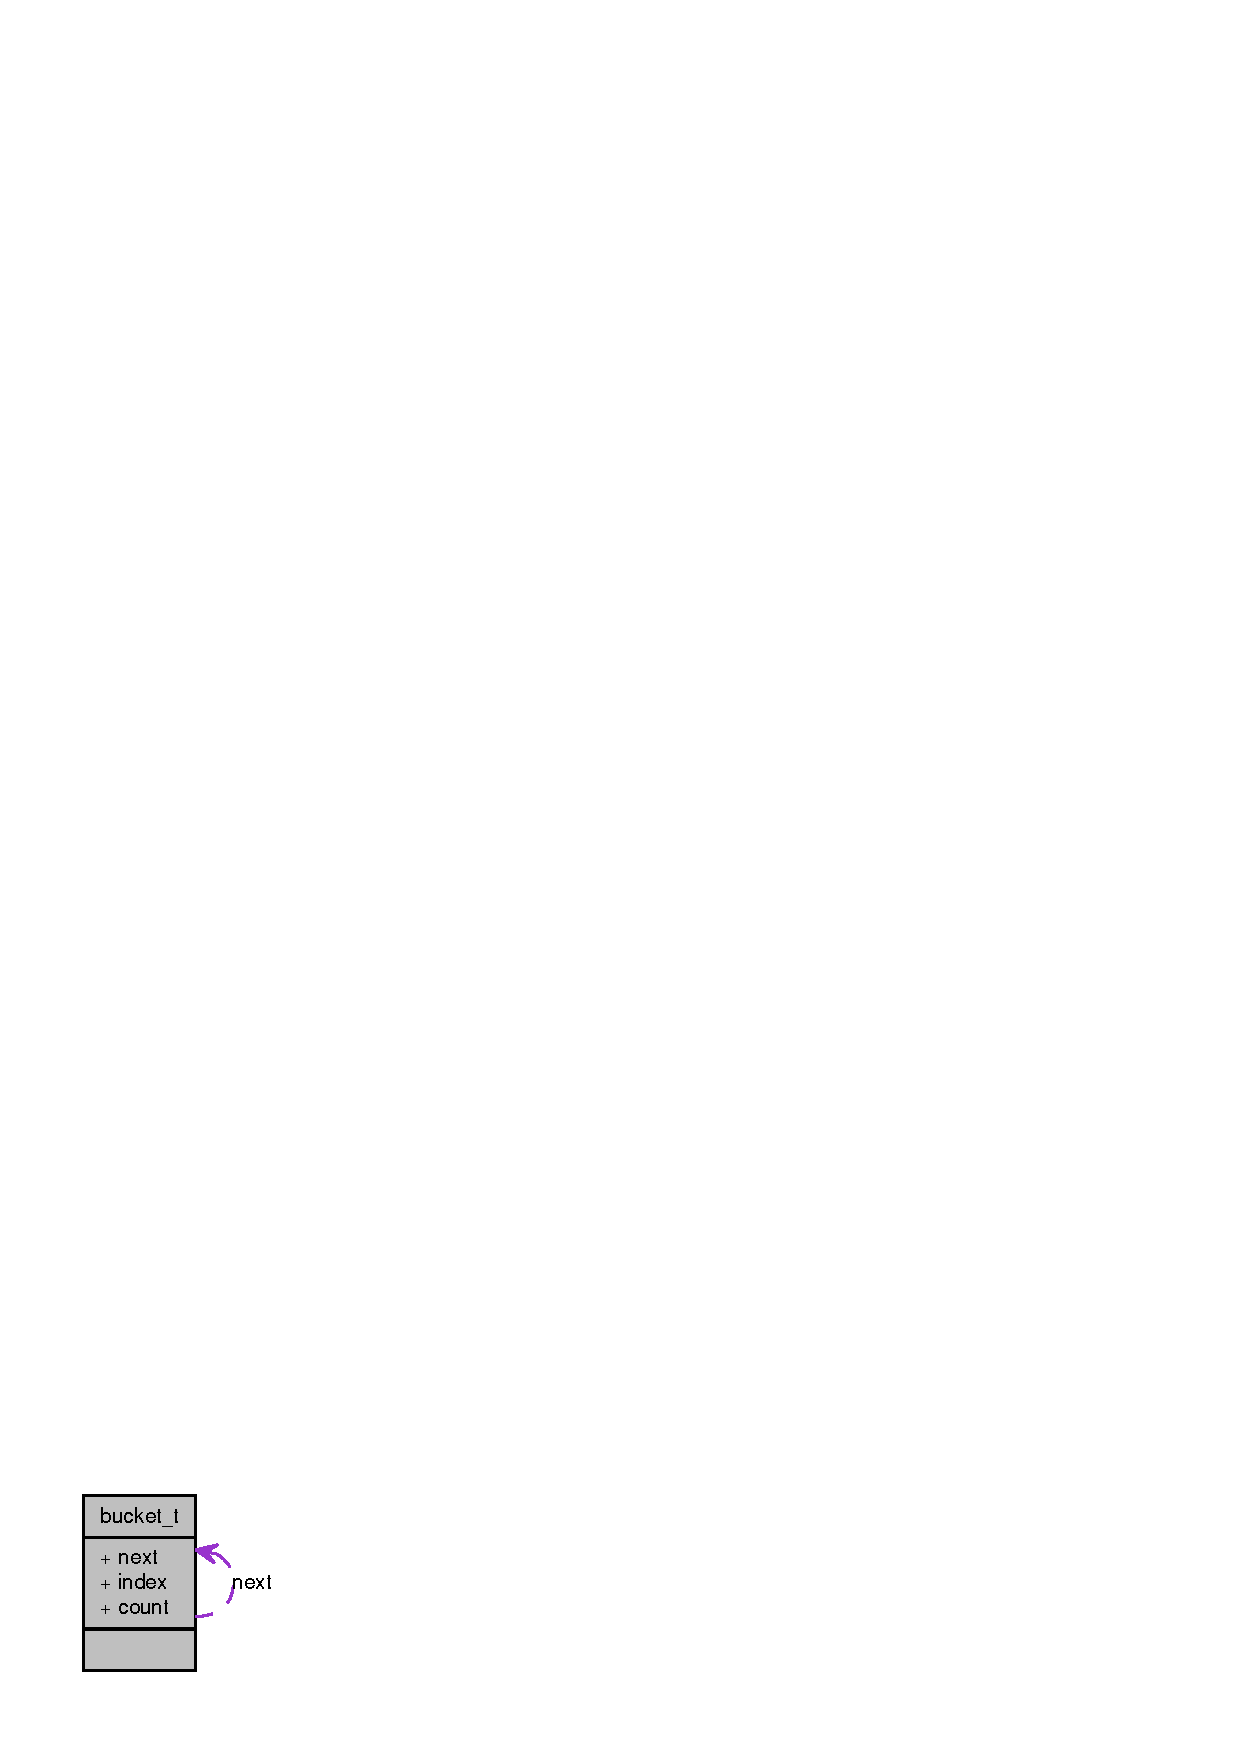
\includegraphics[width=135pt]{structbucket__t__coll__graph}
\end{center}
\end{figure}
\subsection*{Public Attributes}
\begin{CompactItemize}
\item 
struct {\bf bucket\_\-t} $\ast$ {\bf next}
\item 
{\bf md\_\-addr\_\-t} {\bf index}
\item 
unsigned int {\bf count}
\end{CompactItemize}


\subsection{Detailed Description}


Definition at line 96 of file zesto/stats.h.

\subsection{Member Data Documentation}
\index{bucket\_\-t@{bucket\_\-t}!count@{count}}
\index{count@{count}!bucket_t@{bucket\_\-t}}
\subsubsection[{count}]{\setlength{\rightskip}{0pt plus 5cm}unsigned int {\bf bucket\_\-t::count}}\label{structbucket__t_2b62c392a3f40f5ac7d0915ea844130b}




Definition at line 99 of file zesto/stats.h.\index{bucket\_\-t@{bucket\_\-t}!index@{index}}
\index{index@{index}!bucket_t@{bucket\_\-t}}
\subsubsection[{index}]{\setlength{\rightskip}{0pt plus 5cm}{\bf md\_\-addr\_\-t} {\bf bucket\_\-t::index}}\label{structbucket__t_73ae46066728a586dc5ac55431da1d9e}




Definition at line 98 of file zesto/stats.h.\index{bucket\_\-t@{bucket\_\-t}!next@{next}}
\index{next@{next}!bucket_t@{bucket\_\-t}}
\subsubsection[{next}]{\setlength{\rightskip}{0pt plus 5cm}struct {\bf bucket\_\-t}$\ast$ {\bf bucket\_\-t::next}\hspace{0.3cm}{\tt  [read]}}\label{structbucket__t_2c556ac0cf0d2de0d34dec2da5283b98}




Definition at line 97 of file zesto/stats.h.

The documentation for this struct was generated from the following file:\begin{CompactItemize}
\item 
{\bf zesto/stats.h}\end{CompactItemize}
